\section{Application Overview}
In the following chapter a short introduction to the actual system will be given. The general process and the user interface will be presented in \autoref{sub:process}-\ref{sub:ui} and the key areas will be explained. Furthermore an introduction to the underlying database models will be given, which includes the representation of the \gls{SKB} as described in \autoref{sub:SKB}. This is followed by a typical walkthrough to create a new analysis as a clinician. As stated before, the application is available on \href{https://small-data-analyst.herokuapp.com}{https://small-data-analyst.herokuapp.com} and these steps can be reproduced in the demo application. At the end of this chapter a short discussion on observations is included, providing as well the insight feedback of an actual statistician using the software. A detailed view on some key components of the software can be found in \autoref{sec:implementation}.

\subsection{General Process}
\label{sub:process}
The crucial role in the process of enabling clinicians to analyse there clinical data is played by the statistician: registered or approved by an administrator he is allowed to perform significant changes to the \gls{SKB} which is required to provide the clinician with a sophisticated foundation for his analyses. 

To do so a statistician will first prepare the system involving the following steps:


\begin{enumerate}
	\item Defining a research question (see \autoref{fig:ui:rq}).
	\item Assigning suitable models (see \autoref{fig:ui:model}) to a research question and providing assumptions (see \autoref{fig:ui:assumption}) that need to hold to make this model a possible model in a particular analysis.
	\item Defining (global) preferences to express a particular order between models in certain contexts that apply if a certain assumption holds (see \autoref{fig:ui:preference}).
\end{enumerate}

\begin{figure}[h]
\centering
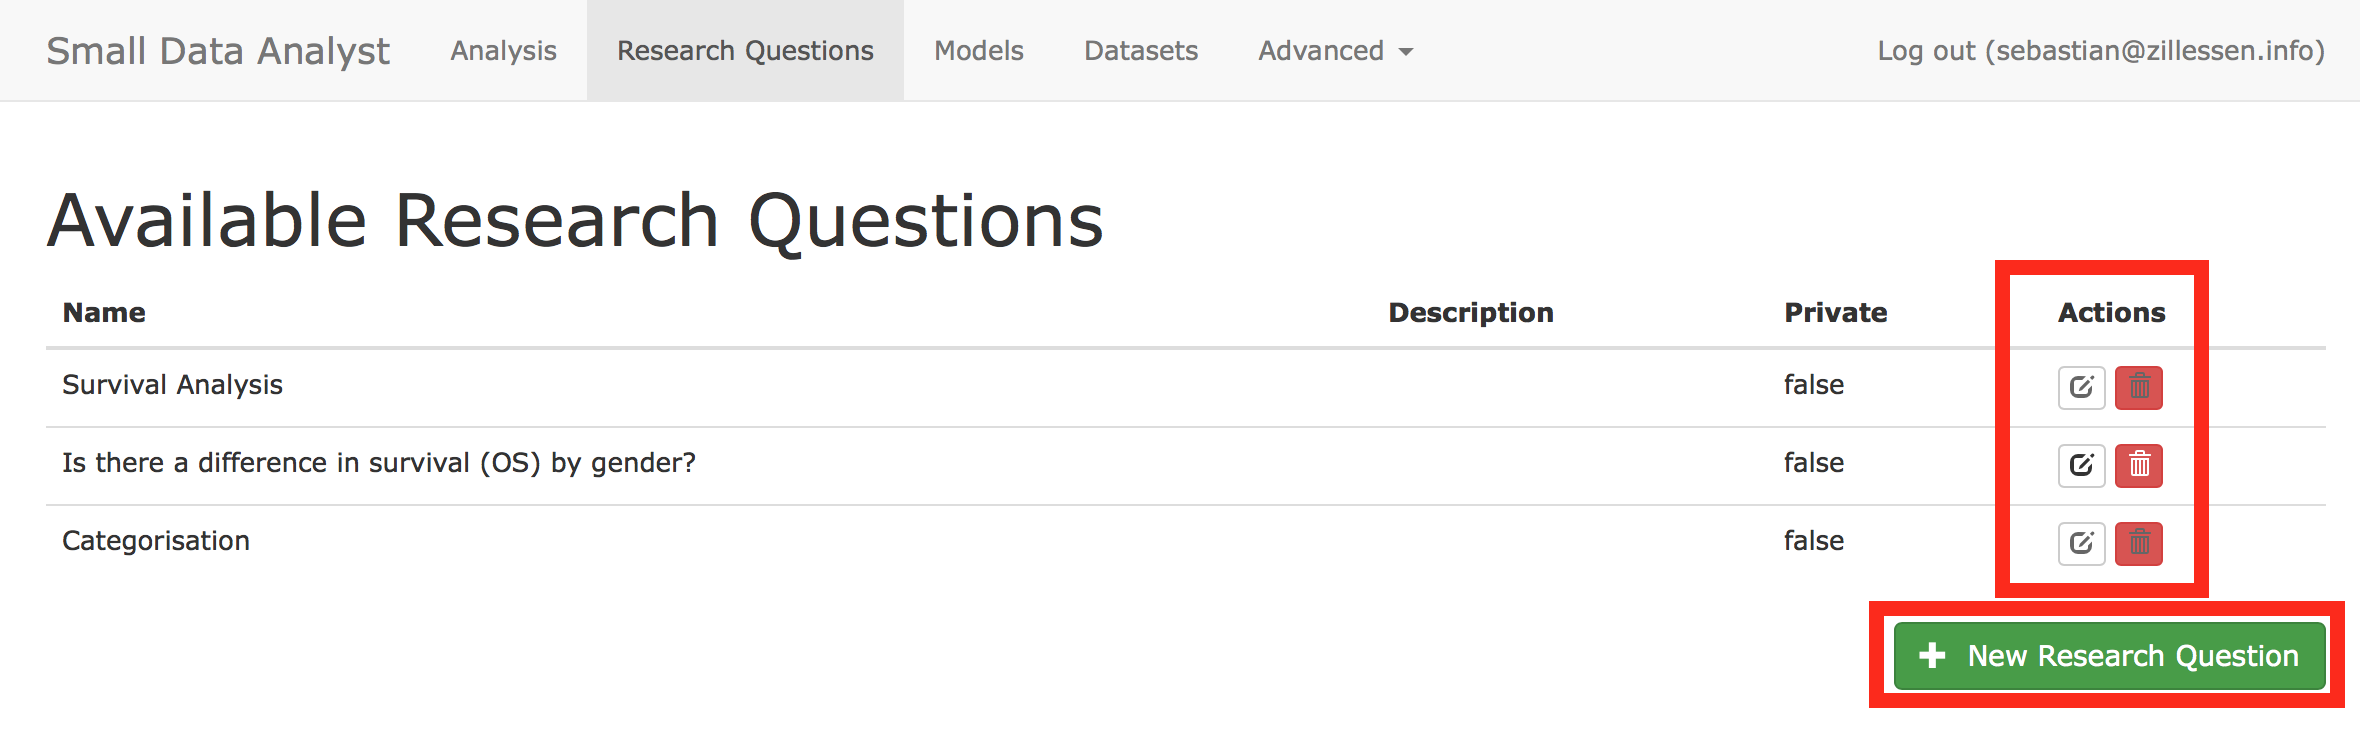
\includegraphics[width=0.8\textwidth]{figures/ui_RQ}
\caption{Listing of research questions: The highlighted areas might not be available, depending on your access rights.}
\label{fig:ui:rq}
\end{figure}


A clinician can then perform a new analysis by performing the steps below:
 
\begin{enumerate}
	\item Uploading a dataset that has been acquired during a clinical study.
	\item Optionally expressing (private) preferences between different models.
	\item Generating a new analysis and providing the answers required by the system to generate a list of possible models.
	\item Answering further data related questions that might arise during the evaluation of the possible models to apply context domain specific preferences on the dataset.
\end{enumerate}

By applying these steps, clinicians will be able to make data-driven decisions that are based on the expertise entered by a statistician.

\subsection{User Interface}
\label{sub:ui}
The \gls{UI} is intentionally kept clean for simplicity reasons: \texttt{Bootstrap} is used to provide a consistent look \& feel and responsiveness of the application. As described in \autoref{sub:sassoon:actors} we have three main users in our system which have different abilities\footnote{Abilities are access rights, that are specified via an \texttt{Ability} class that is used by \texttt{cancancan} to provide diversified access-rights to different user groups in our system.} influencing the appearance of the \gls{UI} (eg. a clinician will not be able to create, alter or delete any research questions, however he will still be able to see them as depicted in \autoref{fig:ui:rq}). This approach allows us to use the same \gls{UI}-components for different users without writing them once again (\gls{DRY} principle).


%\begin{figure}[h]
%\centering
%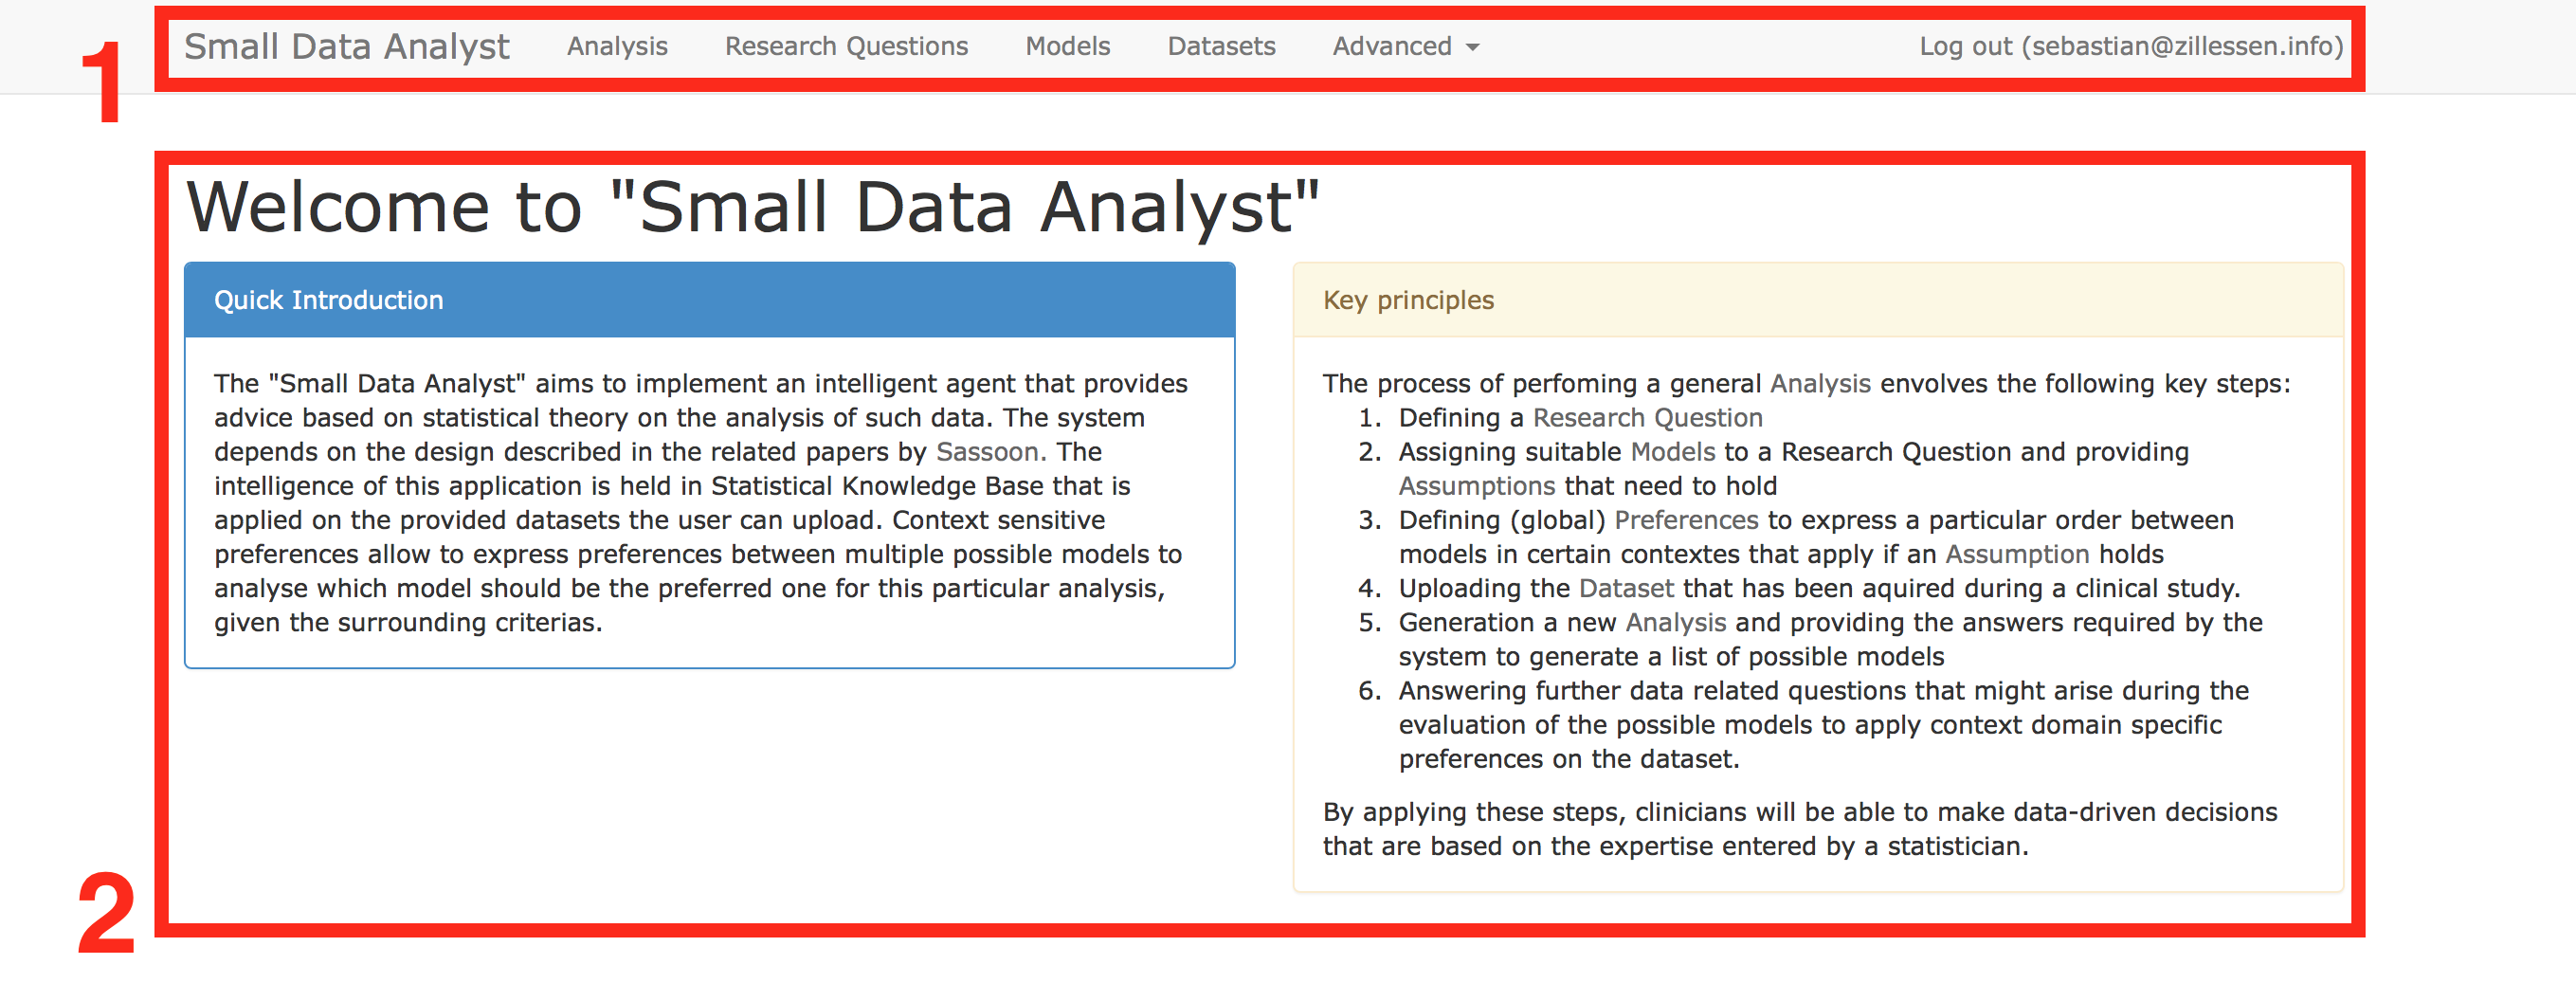
\includegraphics[width=0.8\textwidth]{figures/ui_General}
%\caption{General \gls{UI} of the final application: Navigation bar (1) and Main content area (2).}
%\label{fig:ui:general}
%\end{figure}



\begin{figure}[h]
\centering
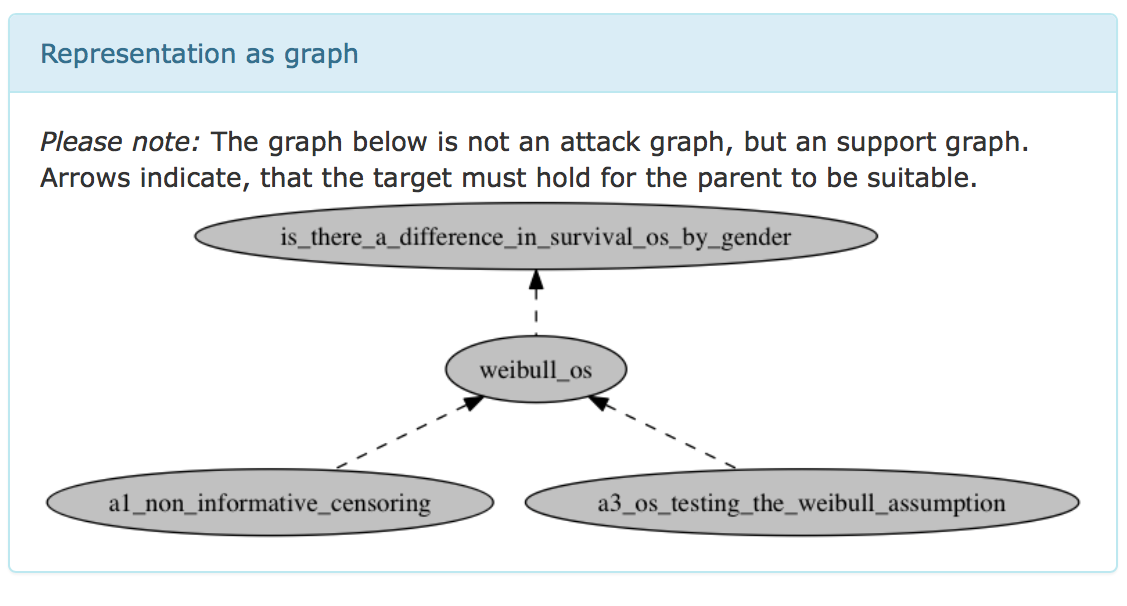
\includegraphics[width=0.8\textwidth]{figures/ui_Weibull_Model}
\caption{Overview over a model, in this particular case the \textit{Weibull model} which requires two assumptions to hold.}
\label{fig:ui:model}
\end{figure}

To provide easier access to the underlying \gls{SKB}, research questions and models include a visual representation of their relations as a graph (see lower right part of\autoref{fig:ui:model}). The system offers four different types of assumptions which have special functionalities (see \autoref{fig:ui:assumption}):

\begin{figure}[h]
\centering
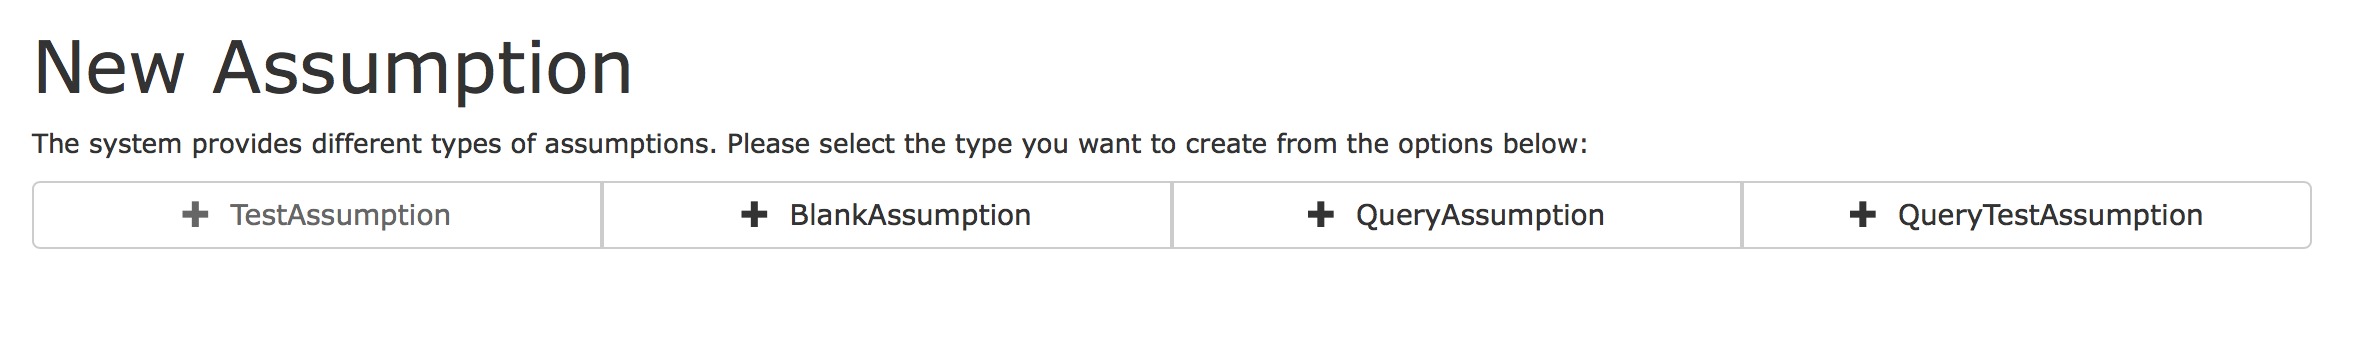
\includegraphics[width=0.8\textwidth]{figures/ui_new_assumption}
\caption{The system provides four different types of assumptions: Test, Query, Test-Query, and Blank assumptions.}
\label{fig:ui:assumption}
\end{figure}


\begin{itemize}
	\item \texttt{TestAssumption}: An assumption that requires a \texttt{R} script to be executed and to return \texttt{true} or \texttt{false}. These assumptions will be checked automatically from the system and rely only on the dataset used in an analysis.
	\item \texttt{QueryAssumption}: A clinician has to provide a \textit{yes} or \textit{no} answer to a question during the process of the analysis. Only if he answers positively, this assumption holds.
	\item \texttt{QueryTestAssumption}: A \texttt{R} script generates a plot based on the dataset, which is then presented to the user who has to confirm that the plot shows some required features.
	\item \texttt{BlankAssumption}: An assumption that represents a grouping ability for other assumptions. It holds only if all of it assigned assumptions (regardless of their type) hold. 
\end{itemize}

Each of those require different attributes which results in different forms during the creation process of new assumptions. 

The most complex component from a \gls{UI} perspective are preferences, as they involve context domains and there required assumptions and relative orders per context domain. \autoref{fig:ui:preference} shows how this has been solved: (1) allows the user to enter general details for a preference (availability to users, rank of the preference and a name). For each context domain that is available for this particular preference (multiple can be added), an assumption (2) has to be chosen. A context domain will be applied, if and only if this assumption holds. The relatively order between models can be specified easily via drag \& drop (3). This order will be taken into account when analysing the \gls{EAF} at the final step of the analysis process. 



\begin{figure}[h]
\centering
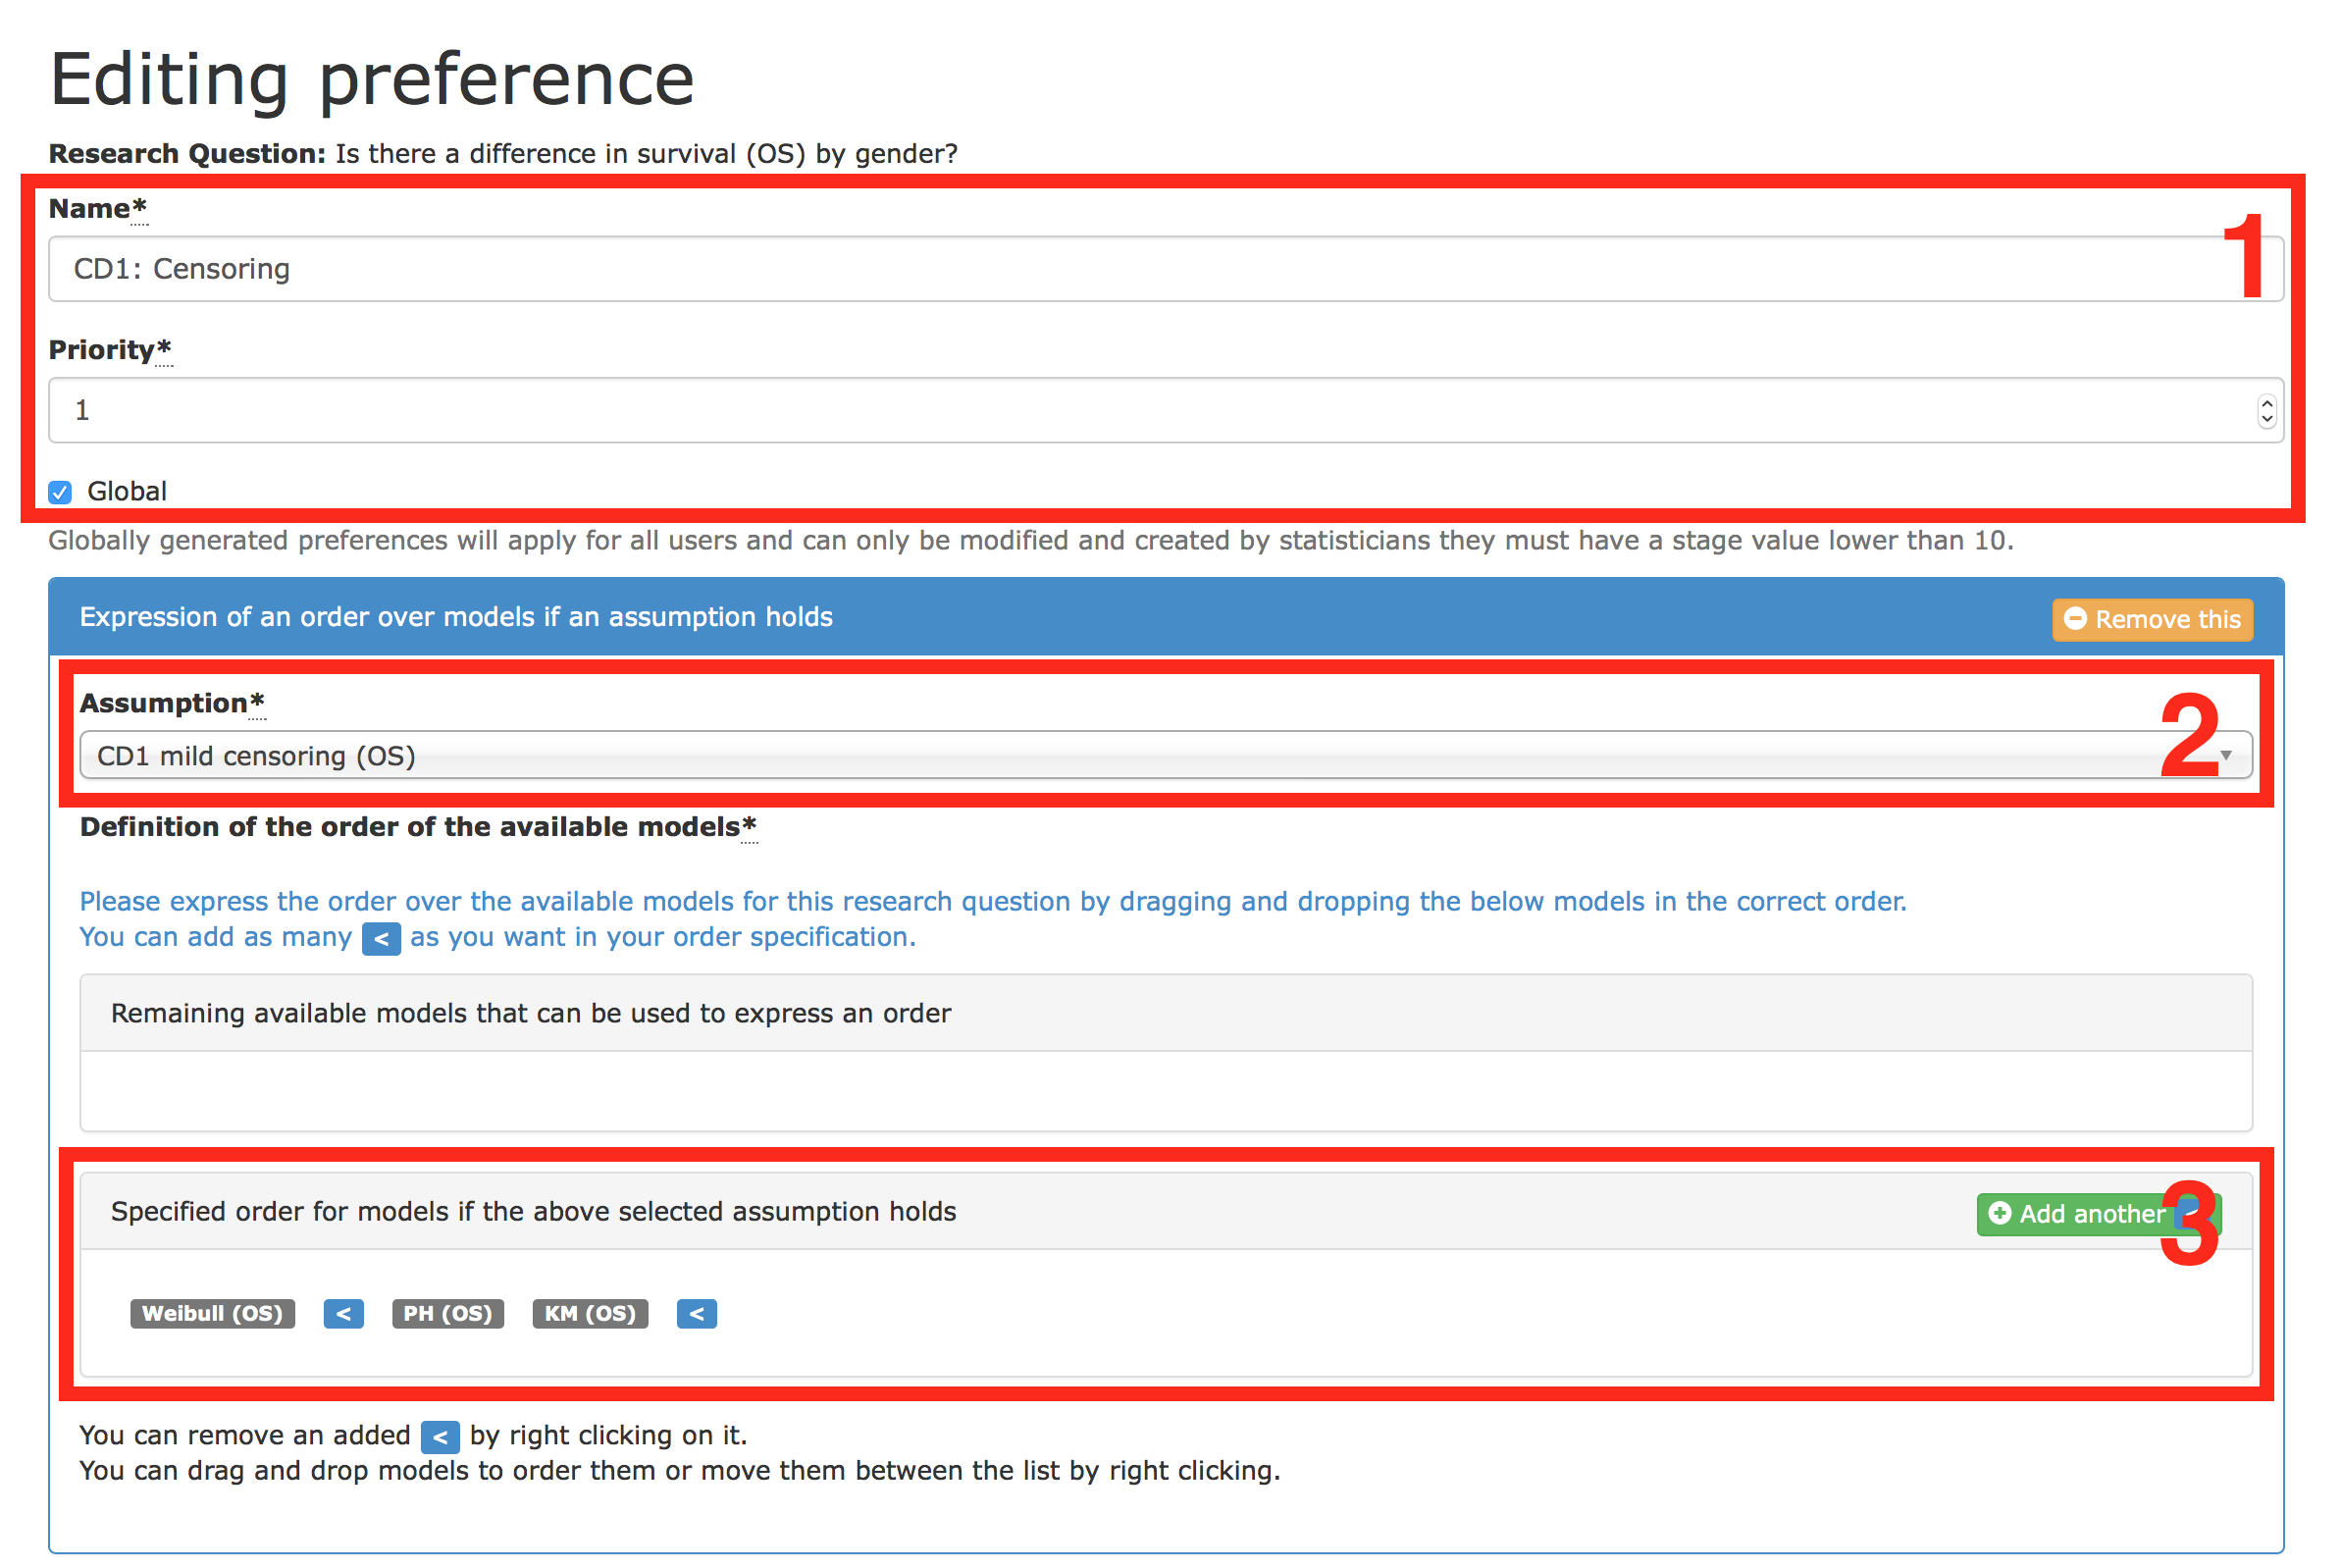
\includegraphics[width=\textwidth]{figures/ui_preference}
\caption{\gls{UI} to enter preferences between models: General information about this preference including the applicable research question (1), the context under which this preference applies can be defined as assumption (2), and the actual order of the models can be interactively arranged per drag \& drop (3).}
\label{fig:ui:preference}
\end{figure}


\subsection{Database models}
\label{sub:db}
\subsection{Example walkthrough}
\label{sub:walk}

\begin{figure}[h]
\centering
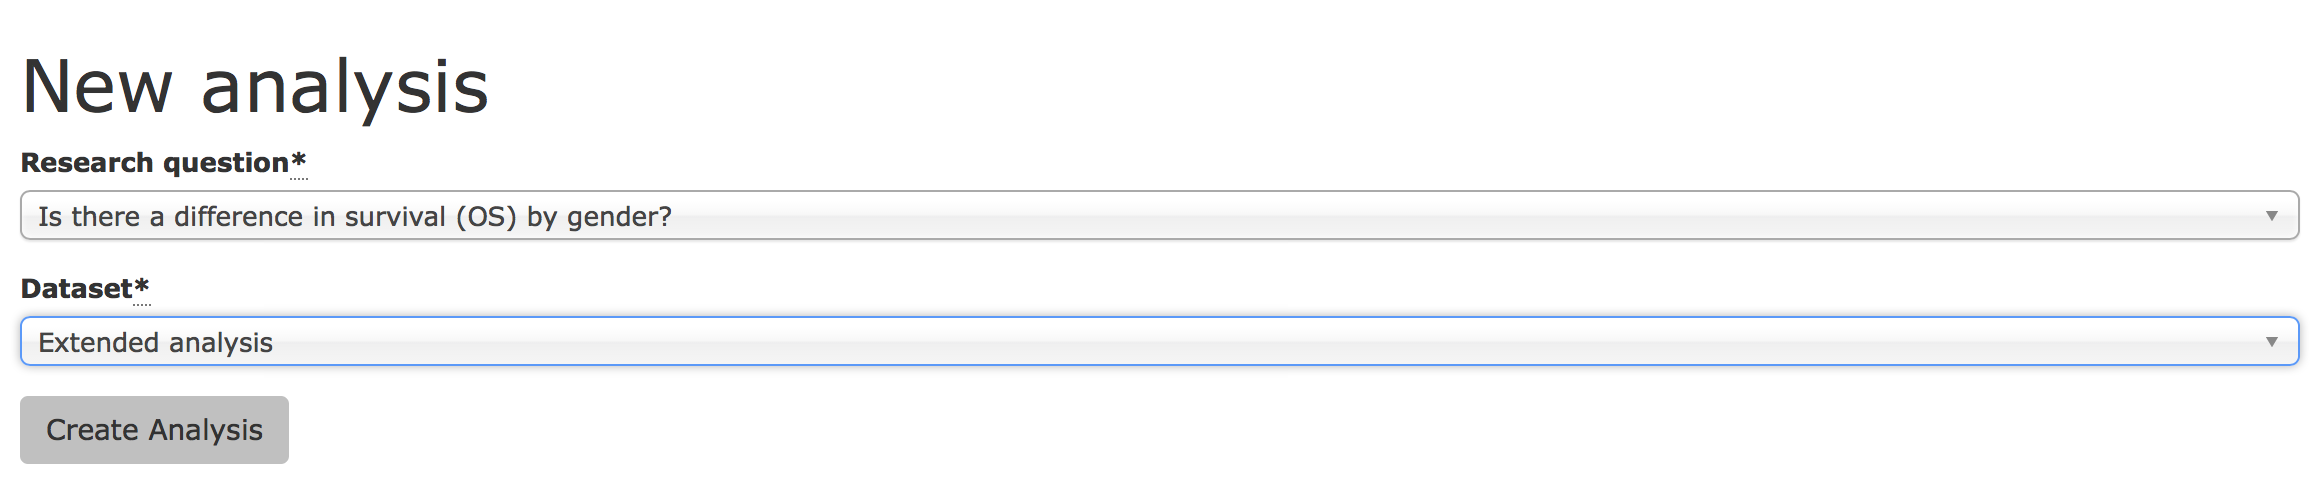
\includegraphics[width=\textwidth]{figures/ui_analysis_0}
\caption{Creating a new analysis, step 1: Selection of dataset and research question. }
\label{fig:analysis:1}
\end{figure}


\begin{figure}[h]
\centering
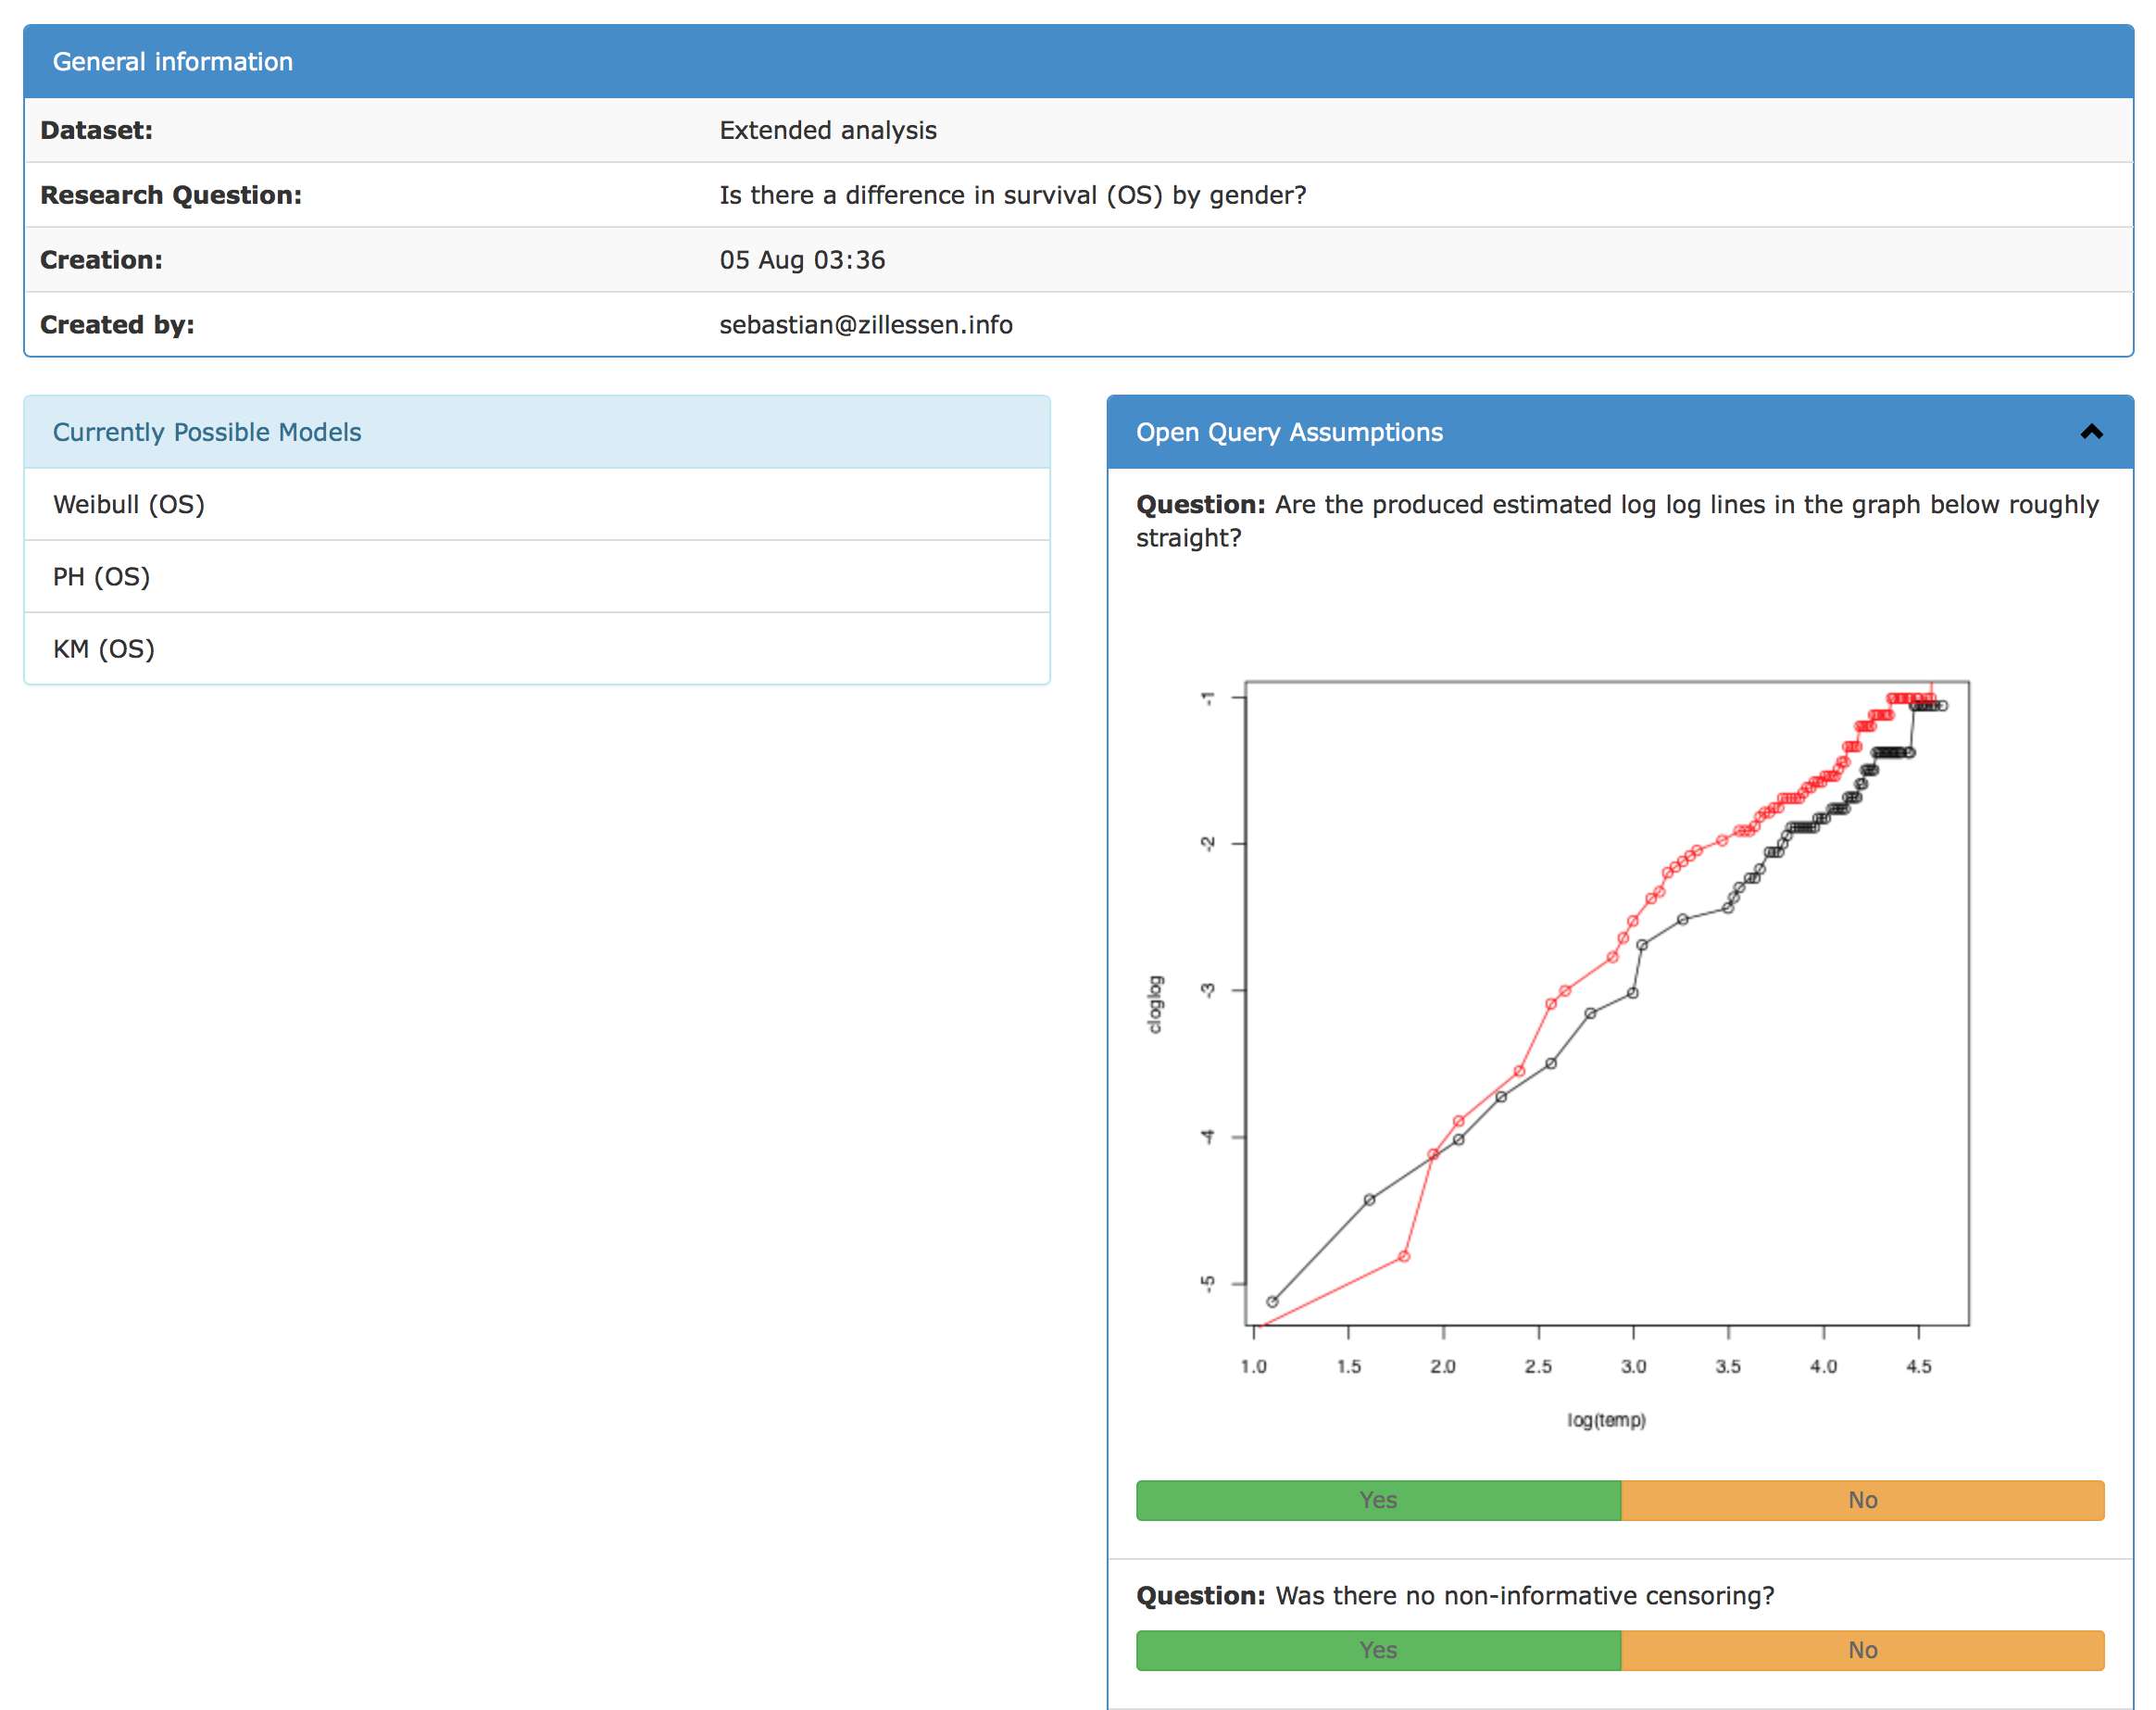
\includegraphics[width=\textwidth]{figures/ui_analysis_1}
\caption{Creating a new analysis, step 2: Clinician has to answer \texttt{QueryTest-} and \texttt{QueryAssumptions} to perform the analysis. \texttt{TestAssumptions} have already been evaluated.}
\label{fig:analysis:2}
\end{figure}

\begin{figure}[h]
\centering
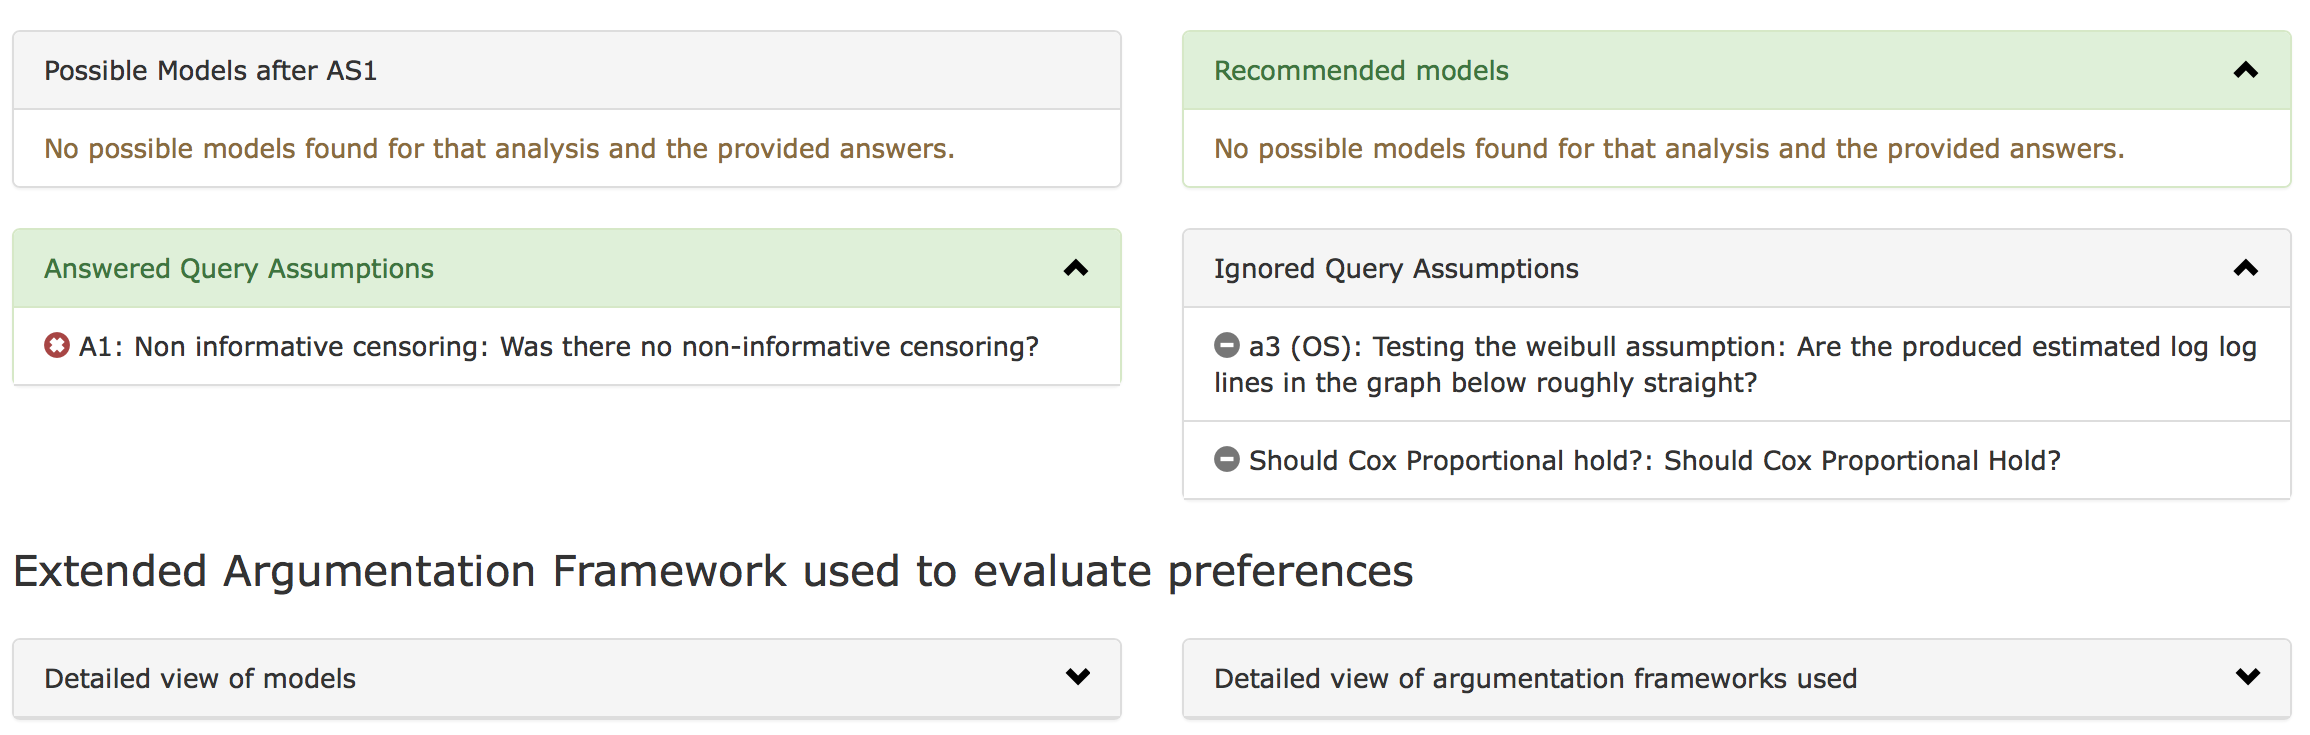
\includegraphics[width=\textwidth]{figures/ui_analysis_2_no}
\caption{Creating a new analysis, step 3: After answering one question (e.g. "Has no non-informative censoring been in place?" with \textit{No}), the possible models are updated and outdated \texttt{QueryAssumptions} might be removed from the list of queries.}
\label{fig:analysis:3_no}
\end{figure}

The picture \autoref{fig:analysis:eaf} shows an analysis performed involving the dataset XXX\todo{describe dataset} and a survival analysis by gender, where the preferences have been set according to \cite{sassoon2016CD}. All \texttt{QueryAssumptions} have been answered positively, so after the initial initialisation of the argumentation framework all three models remain possible. During the evaluation of the preferences per context domain \textit{Kaplan-Meier} and \textit{Weibull} models are wiped-out as "\textit{Censoring}" has the performance measurement \textbf{heavy}. The generated \gls{EAF} on the right side of \autoref{fig:analysis:eaf} shows the reason why only \textit{Cox-Proportional hazard} remains as the last preferred model.

\begin{figure}[h]
\centering
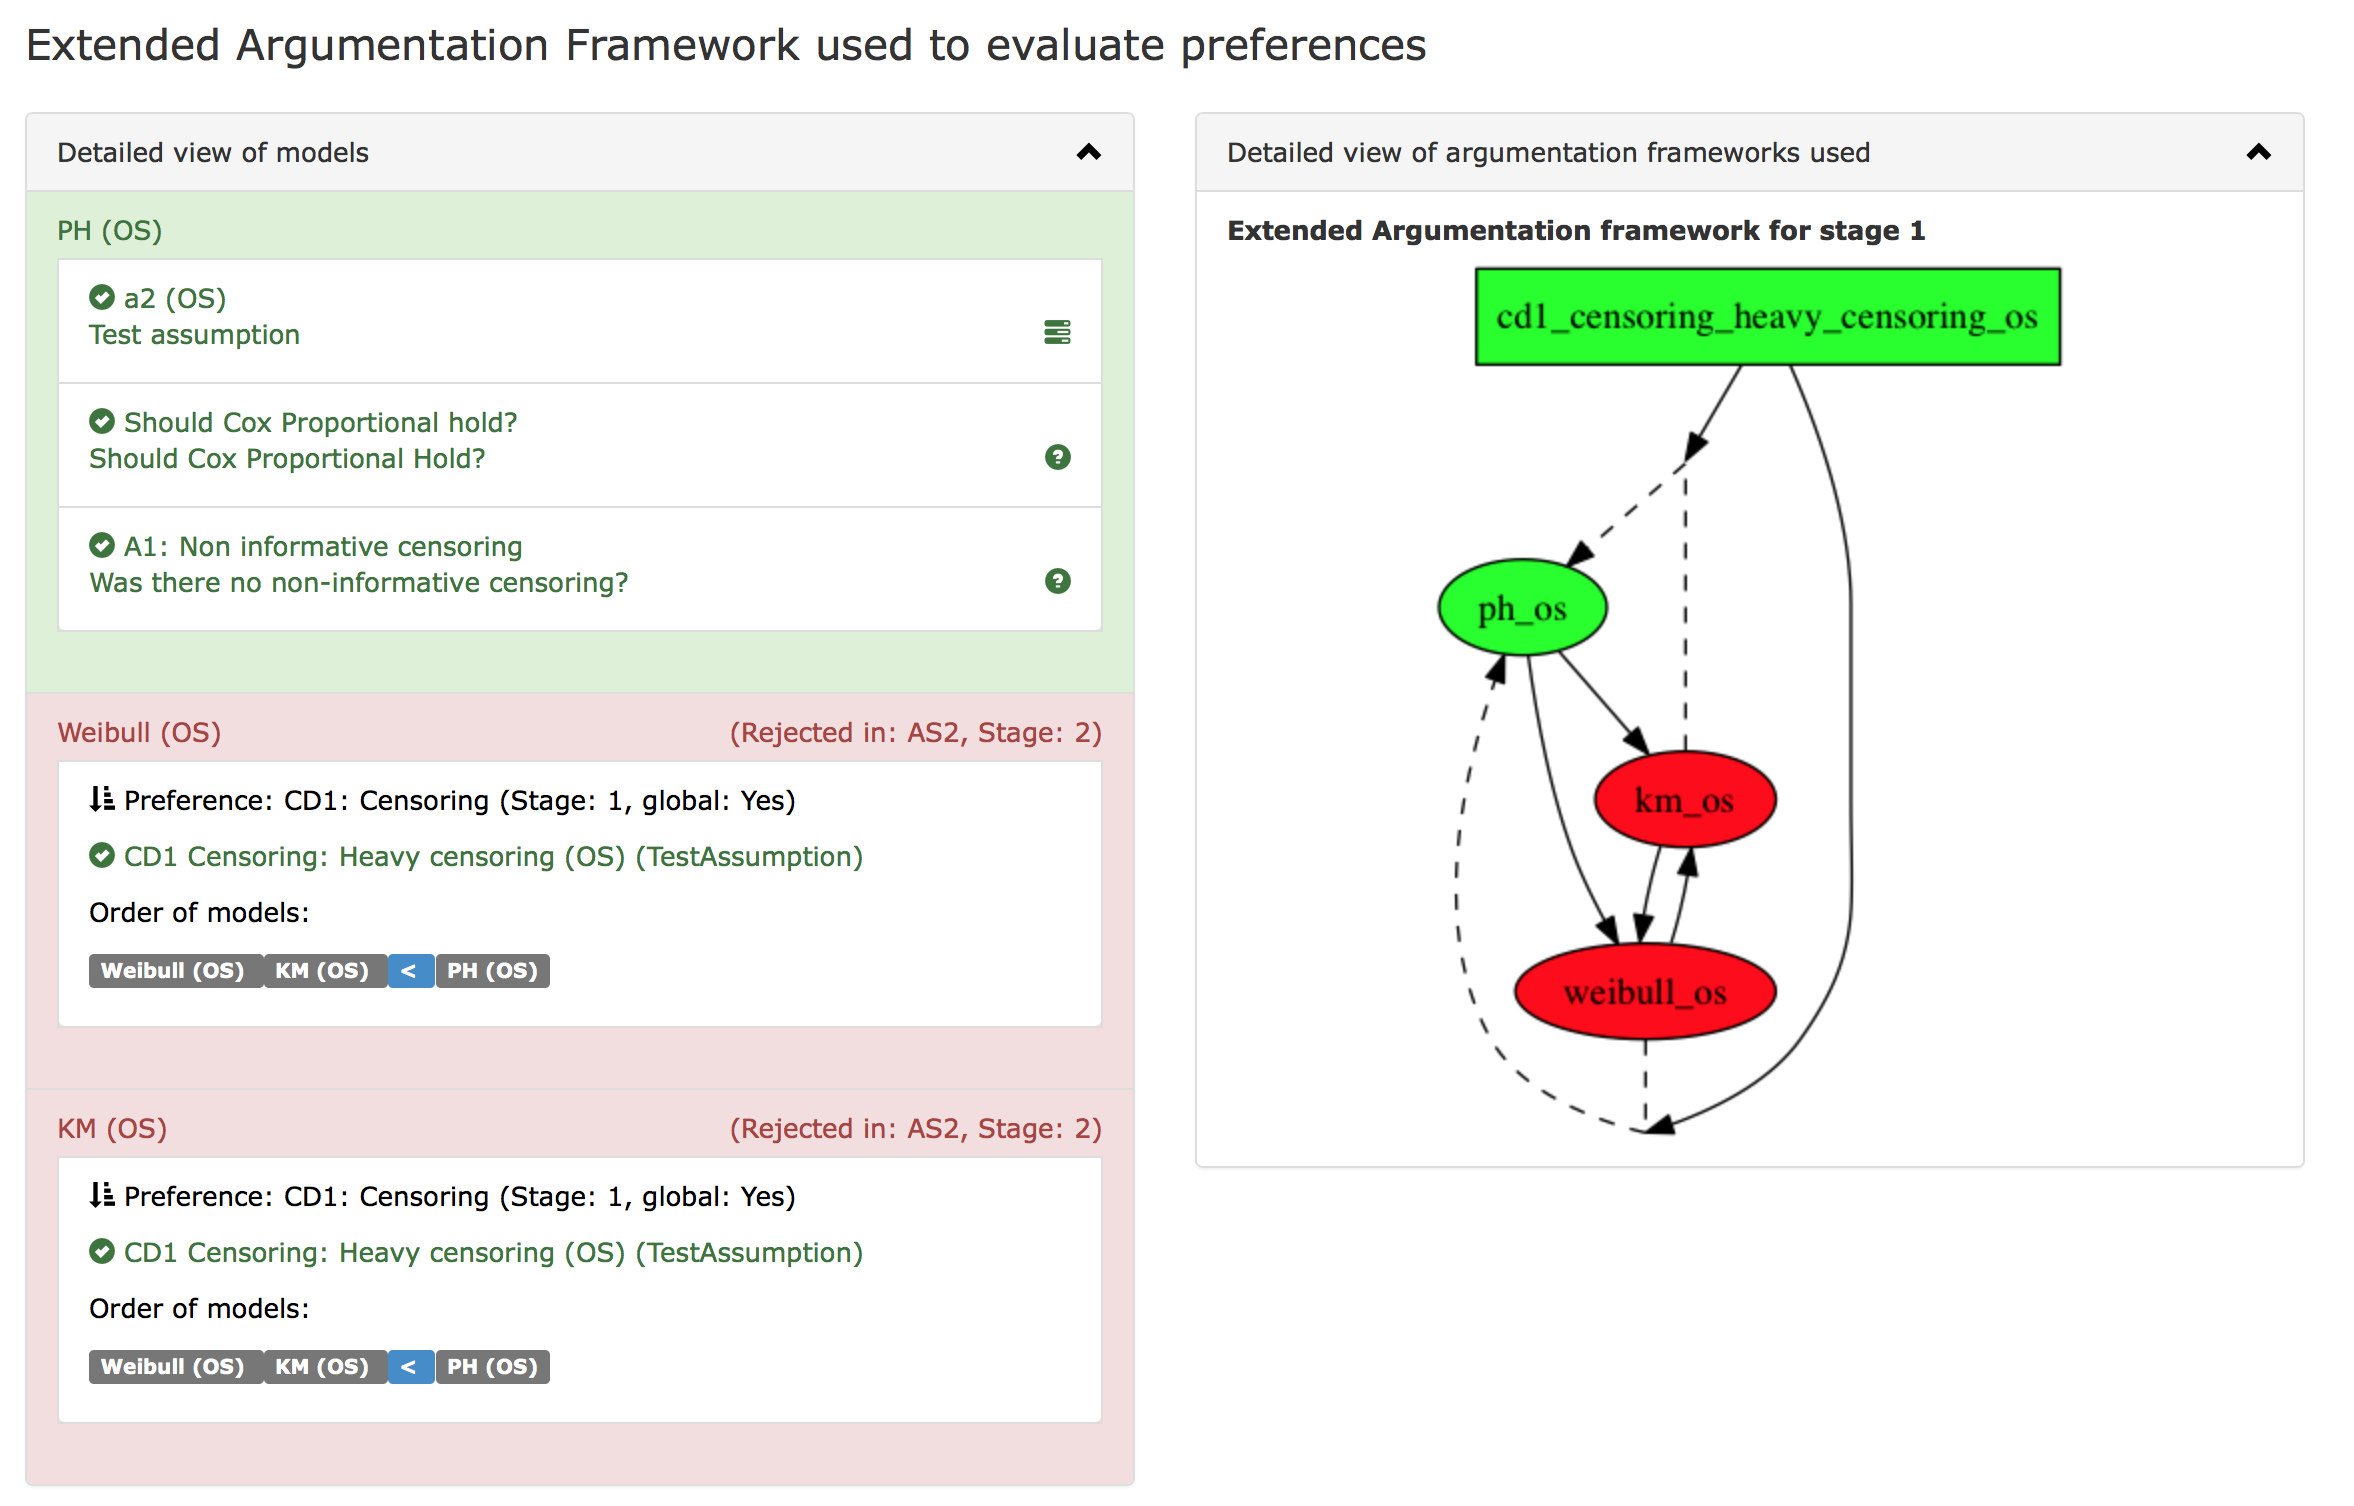
\includegraphics[width=\textwidth]{figures/ui_analysis_eaf}
\caption{Finished analysis with applied preferences on it: context domain "Censoring" evaluated to \textit{heavy censoring}. }
\label{fig:analysis:eaf}
\end{figure}

\subsection{Observation and Discussion}
\todo{feedback of an actual statistician}



\todo{Main Result:  The chapter reports the contribution of your work.  For example, it could contain the following sub-sections to summarise the contribution of the project: Theoretical Development, Analysis and Design, Implementation and Experimental Work, Results, Observation and Discussion.}